\documentclass[a4paper,12pt]{article}
\usepackage{amssymb}
\usepackage{amsmath}
\usepackage[utf8]{inputenc} % Umlaute
\usepackage[ngerman]{babel} % Umlaute
\usepackage[T1]{fontenc}    % Umlaute
\usepackage[margin=2.5cm]{geometry}
\usepackage{booktabs}
\usepackage{lmodern}
\usepackage{titlesec}
\usepackage{longtable}
% Notwendig für Links im Text
\usepackage{hyperref}
\usepackage[table]{xcolor}% http://ctan.org/pkg/xcolor
%%\usepackage{svg}
% glossar, see http://en.wikibooks.org/wiki/LaTeX/Glossary
% muss NACH hyperref geladen werden, sonst funktionieren die Links nicht
\usepackage[toc]{glossaries}

% Kompatibilität
\ifx\pdftexversion\undefined
\usepackage[dvips]{graphicx}
\else
\usepackage[pdftex]{graphicx}
\DeclareGraphicsRule{*}{mps}{*}{}
\fi
\setlength{\parindent}{0pt}
\usepackage{subfigure}
\usepackage{placeins}

%valle will Automaten verwenden
\usepackage{tikz}
\usetikzlibrary{automata, positioning, arrows}

%irgendwas mit section formatierung (titlesec package)
\titleformat{\paragraph}[hang]{\normalfont\normalsize\bfseries}{\theparagraph}{1em}{}
%%%%%%%%%%%%%%%%%%%%%%%%%%%%%%%%%%%%%%%%%%%%%%%%%%%%%%%%%%%%%%%%%%%%%%
% Variablen                                 						 %
%%%%%%%%%%%%%%%%%%%%%%%%%%%%%%%%%%%%%%%%%%%%%%%%%%%%%%%%%%%%%%%%%%%%%%
\newcommand{\authorName}{Tec O'Brain (Entwickler: David Höglinger, Jan Ettrich, Erwin Müller, Benedikt Rittner, Valentin Quapil)}
\newcommand{\auftraggeber}{Karlsruhe Institute of Technology (Teco)}
\newcommand{\auftragnehmer}{\authorName}
\newcommand{\projektName}{Validierung Earables}
\newcommand{\tags}{\authorName, Validierung, Tests, KIT, Informatik, PSE}
\newcommand{\documentVersion}{1.0}
\title{\projektName}
\date{\today}
\author{Tec O'Brain}

%%%%%%%%%%%%%%%%%%%%%%%%%%%%%%%%%%%%%%%%%%%%%%%%%%%%%%%%%%%%%%%%%%%%%%
% PDF Meta information                                 				 %
%%%%%%%%%%%%%%%%%%%%%%%%%%%%%%%%%%%%%%%%%%%%%%%%%%%%%%%%%%%%%%%%%%%%%%
\hypersetup{
  pdfauthor   = {\authorName},
  pdfkeywords = {\tags},
  pdftitle    = {\projektName)}
}

%%%%%%%%%%%%%%%%%%%%%%%%%%%%%%%%%%%%%%%%%%%%%%%%%%%%%%%%%%%%%%%%%%%%%%
% Create a shorter version for tables. DO NOT CHANGE               	 %
%%%%%%%%%%%%%%%%%%%%%%%%%%%%%%%%%%%%%%%%%%%%%%%%%%%%%%%%%%%%%%%%%%%%%%
\newcommand\addrow[2]{#1 &#2\\ }

\newcommand\addheading[2]{#1 &#2\\ \hline}
\newcommand\tabularhead{\begin{tabular}{lp{13cm}}
\hline
}

\newcommand\addmulrow[2]{ \begin{minipage}[t][][t]{2.5cm}#1\end{minipage}%
   &\begin{minipage}[t][][t]{8cm}
    \begin{enumerate} #2   \end{enumerate}
    \end{minipage}\\ }

\newcommand{\testok}[0]{
	\cellcolor{green!25} OK
}

\newcommand{\testntb}[0]{NTB}

\newcommand{\testfailed}[0]{
	\cellcolor{red!25} FAILED
}

\newenvironment{usecase}{\tabularhead}
{\hline\end{tabular}}

\usepackage{microtype}
%%%%%%%%%%%%%%%%%%%%%%%%%%%%%%%%%%%%%%%%%%%%%%%%%%%%%%%%%%%%%%%%%%%%%%
% GLOSSARY ENTRIES                 	                              	 %
%%%%%%%%%%%%%%%%%%%%%%%%%%%%%%%%%%%%%%%%%%%%%%%%%%%%%%%%%%%%%%%%%%%%%%


%%%%%%%%%%%%%%%%%%%%%%%%%%%%%%%%%%%%%%%%%%%%%%%%%%%%%%%%%%%%%%%%%%%%%%
% THE DOCUMENT BEGINS             	                              	 %
%%%%%%%%%%%%%%%%%%%%%%%%%%%%%%%%%%%%%%%%%%%%%%%%%%%%%%%%%%%%%%%%%%%%%%
\begin{document}
\pagenumbering{roman}
\begin{titlepage}
\maketitle
\thispagestyle{empty} % no page number

\begin{verbatim}












\end{verbatim}


  \begin{tabular}[t]{p{4 cm}p{8 cm}}
	Projekt:       & \projektName \\[1.2ex]
	Auftraggeber:  & \auftraggeber\\[1.2ex]
	Auftragnehmer: & \auftragnehmer\\[1.2ex]
  \end{tabular}


\begin{tabular}[t]{|p{4 cm}|p{8 cm}|}
\hline
\textbf{Datum} & \textbf{Autor(en)} \\
\hline
\hline
\today & \authorName \\
\hline
\end{tabular}
\end{titlepage}
         % Deckblatt.tex laden und einfügen
\setcounter{page}{2}
\tableofcontents          % Inhaltsverzeichnis ausgeben
\clearpage
\pagenumbering{arabic}
%%%%%%%%%%%%%%%%%%%%%%%%%%%%%%%%%%%%%%% CONTENT %%%%%%%%%%%%%%%%%%%%%%%%%%%%%%%%%%%%%%%%%%%%%%%

\section{Einleitung}
In diesem Dokument wird festgehalten, wie zuverlässig und vor allem wie korrekt der Code ist, den wir in der Implementierungsphase angefertigt haben.
Dabei kommen die Testszenarien, die wir im Pflichtenheft spezifiziert haben, zum Einsatz und helfen uns dabei, die Korrektheit unserer App zu sichern.
Zusätzlich wurden xUnit-Tests geschrieben, welche große Bereiche unseres Codes abdecken.\\
Die Codecoverage wurde mit ReSharper ermittelt und im Dokument durch aussagekräftige Diagramme visualisiert.
Für unsere Bibliothek haben wir zusätzlich eine Test App geschrieben, die uns mit neu angefertigten Szenarien dabei hilft, die Korrektheit sicher zu stellen.\\
Außerdem haben wir 5 Probanden gefunden, die sich bereiterklärt haben, unsere App auszuprobieren.
Mit Hilfe ihrer Kritik und ihren Anmerkungen konnten wir die App noch nutzerfreundlicher und besser machen.
\section{Testszenarien}

%Table template:
\iffalse
\begin{tabular}{ |p{1.5cm} | p{12cm} | c| }
	\hline
	\textbf{Testfall} & \textbf{Beschreibung} & \textbf{Bestanden}\\
	\hline
	/T070/ & Der Nutzer startet die App. & \testok\\
	\hline	
\end{tabular}
\fi
\paragraph{Einleitung}
Die Testszenarien setzen sich aus den im Pflichtenheft genannten Testfällen (T) zusammen.
Die Testszenarien wurden schon vor der Entwicklung festgelegt (in der Definitionsphase), alle Änderungen an den Szenarien werden im Folgenden vor dem entsprechenden Szenario erwähnt.
\\
Die Überdeckung der Szenarientests beträgt 98,75\%.\\
Erfolgreich waren 92,5\% der insgesamt 80 Tests.

\paragraph{Legende} 
\begin{itemize}
	\item OK: In allen Testläufen erfolgreich
	\item FAILED: In mindestens einem Testlauf nicht erfolgreich
	\item NTB: Konnte nicht getestet werden
\end{itemize}
\clearpage
\subsection{Laufmodus}
\begin{tabular}{ |p{1.5cm} | p{12cm} | c| }
	\hline
	\textbf{Testfall} & \textbf{Beschreibung} & \textbf{Bestanden}\\
	\hline
	/T070/ & Der Nutzer startet die App. & \testok \\
	\hline
	/T140/ & Der Nutzer verbindet in der App die Earables, über BLE mit seinem Smartphone. & \testok \\
	\hline
	/T070/ & Nach dem Startvorgang der App wird in den Modus \glqq Laufmodus\grqq{} gewechselt. & \testok \\
	\hline
	/T104/ & Falls es schon einen Laufvorgang zuvor gab, werden nun die Anzahl der zurückgelegten Schritte und die zurückgelegte Distanz angezeigt.& \testok \\
	\hline
	& Die Earables werden korrekt am Ohr des Nutzers angebracht. & \testok \\
	\hline
	/T075/ & Der Nutzer startet den Laufmodus. & \testok \\
	\hline
	/T100/ & Die App zeigt dem Nutzer den Status \glqq stehend\grqq{} an. & \testok \\
	\hline
	/T101/ & Die App zeigt dem Nutzer die aktuelle Schrittfrequenz und die Anzahl der bisher gegangenen Schritte. & \testok \\
	\hline
	/T100/ & Sobald der Nutzer anfängt zu gehen zeigt die App \glqq gehend\grqq{} an. & \testok \\
	\hline
	/T100/ & Sobald der Nutzer wieder still steht ändert sich der Zustand wieder zurück zu \glqq stehend\grqq. & \testok \\
	\hline	
\end{tabular}


\subsection{Zählmodus}
\begin{tabular}{ |p{1.5cm} | p{12cm} | c| }
	\hline
	\textbf{Testfall} & \textbf{Beschreibung} & \textbf{Bestanden}\\
	\hline
	/T070/ & Der Nutzer startet die App. & \testok \\
	\hline
	/T140/ & Der Nutzer verbindet in der App die Earables, über BLE mit seinem Smartphone. & \testok \\
	\hline
	/T090/ & Nach dem Startvorgang der App wechselt der Nutzer in den Modus \glqq Zählmodus\grqq . & \testok \\
	\hline
	& Die Earables werden korrekt am Ohr des Nutzers angebracht. & \testok  \\
	\hline
	/T200/ & Der Nutzer wählt eine verfügbare Übung aus. & \testok  \\
	\hline
	/T075/ & Der Nutzer startet den gewählten Vorgang. & \testok  \\
	\hline
	/T170/, /T180/ & Der Nutzer führt die Übung 15 (natürliche Zahl) mal aus. & \testok  \\
	\hline
	/T080/ & Der Nutzer stoppt den laufenden Vorgang. & \testok  \\
	\hline
	/T200/ & Die App zeigt 15 an. & \testfailed  \\
	\hline
\end{tabular}
\paragraph{Anmerkungen}
Die App zeigte in 2 von 3 Fällen am Ende nich exakt 15 an.\\
Im ersten Fall (bei SitUps) wurden nur 10 erkannt, im zweiten Fall (bei Liegestützen) wurde eine Liegestütze doppelt erkannt. 
\clearpage
\subsection{Start/Stop Musikmodus}
\paragraph{Änderungen}
Die Funktion wurde aus dem Laufmodus in den Modus \glqq Musik Modus\grqq{} umbenannt.
\\
\\
\begin{tabular}{ |p{1.5cm} | p{12cm} | c| }
	\hline
	\textbf{Testfall} & \textbf{Beschreibung} & \textbf{Bestanden}\\
	\hline
	/T070/ & Der Nutzer startet die App. & \testok \\
	\hline
	/T140/ & Der Nutzer verbindet in der App die Earables, über BLE mit seinem Smartphone. & \testok \\
	\hline
	& Der Nutzer spielt Musik mit der vorinstallierten Musik-App ab. & \testntb \\
	\hline
	/T090/ & Nach dem Startvorgang der App wechselt der Nutzer in den Modus \glqq Music Mode\grqq . & \testok \\
	\hline
	& Die Earables werden korrekt am Ohr des Nutzers angebracht. & \testok \\
	\hline
	& Der Nutzer beginnt zu gehen. & \testok  \\
	\hline
	/T075/ & Der Nutzer startet den gewählten Vorgang. & \testok  \\
	\hline
	& Der Nutzer hört auf zu gehen. & \testok  \\
	\hline
	/T210/ & Die Musik wird pausiert. & \testok  \\
	\hline
	& Der Nutzer geht weiter. & \testok  \\
	\hline
	/T210/ & Die Musik startet automatisch wieder. & \testok  \\
	\hline
\end{tabular}
\paragraph{Anmerkungen}
Das Abspielen der Musik wurde in der Implemetierungsphase nicht über eine externe Musik-App realisiert (siehe Implementierungsprotokoll). 

\subsection{Lauschen\&Agieren}
\paragraph{Änderungen}
Der Lauschen\&Agieren Modus wird nicht mehr automatisch beendet, sondern durch den Nutzer.  
\\
\\
\begin{tabular}{ |p{1.5cm} | p{12cm} | c| }
	\hline
	\textbf{Testfall} & \textbf{Beschreibung} & \textbf{Bestanden}\\
	\hline
	/T070/ & Der Nutzer startet die App. & \testok \\
	\hline
	/T140/ & Der Nutzer verbindet in der App die Earables, über BLE mit seinem Smartphone. & \testok  \\
	\hline
	/F090/ & Nach dem Startvorgang der App wechselt der Nutzer in den Modus \glqq Lauschen\&Agieren\grqq . & \testok  \\
	\hline
	& Die Earables werden korrekt am Ohr des Nutzers angebracht. & \testok  \\
	\hline
	/T221/ & Der Nutzer stellt sich ein Training aus den verfügbaren Übungen zusammen. & \testok  \\
	\hline
	& Der Nutzer startet den gewählten Vorgang. & \testok  \\
	\hline
	/T222/ & Dem Nutzer wird per Text-To-Speech die aktuelle Übung angesagt. & \testok  \\
	\hline
	& Der Nutzer führt die Übung aus. & \testok  \\
	\hline
	/T222/ & Die letzten beiden Schritte werden so lange wiederholt, bis alle ausgewählten Übungen erledigt sind. & \testok  \\
	\hline
	& Der Vorgang wird automatisch beendet. & \testfailed \\
	\hline
	/T223/ & Die App zeigt die benötigte Zeit für den Vorgang an. & \testok  \\
	\hline
\end{tabular}
\subsection{Einstellungen}
\paragraph{Änderungen}
Die Standardsprache ist Englisch, daher wurde /T260/ auf Deutsch geändert.\\
Das Löschen der Vorgangsdaten wurde auf eine andere Seite in der App verlegt.
\\
\\
\begin{tabular}{ |p{1.5cm} | p{12cm} | c| }
	\hline
	\textbf{Testfall} & \textbf{Beschreibung} & \textbf{Bestanden}\\
	\hline
	/T070/ & Der Nutzer startet die App. & \testok \\
	\hline
	/T140/ & Der Nutzer verbindet in der App die Earables, über BLE mit seinem Smartphone. & \testok  \\
	\hline
	/T090/ & Nach dem Startvorgang der App wechselt der Nutzer in die Ansicht \glqq Einstellungen\grqq . & \testok \\
	\hline
	/T250/ & Der Nutzer ändert seinen Namen. & \testok  \\
	\hline
	/T260/ & Der Nutzer ändert die Sprache auf Deutsch & \testok  \\
	\hline
	/T270/ & Dem Nutzer löscht die gespeicherten Vorgangsdaten. & \testfailed  \\
	\hline
	/T280/ & Dem Nutzer ändert die Samplingrate & \testok  \\
	\hline
	/T285/ & Der Nutzer ändert seine Schrittlänge. & \testok  \\
	\hline
	& Der Nutzer klickt auf speichern. & \testok  \\
	\hline
	& Der Nutzer beendet die App. & \testok  \\
	\hline
	/T070/ & Der Nutzer startet die App. & \testok  \\
	\hline
	/T090/ & Der Nutzer wechselt in die Ansicht \glqq Einstellungen\grqq . & \testok  \\
	\hline
	& Die Einstellungen sind exakt so, wie sie vorher eingestellt wurden. & \testfailed  \\
	\hline
\end{tabular}
\paragraph{Anmerkungen}
Die Samplerate wurde nicht gespeichert. Dieser Bug wurde behoben.

\subsection{Erstnutzung}
\paragraph{Änderungen}
Der Punkt \glqq Der Nutzer klickt auf SAVE\grqq{} wurde hinzugefügt. Außerdem wurde die Sprache von Englisch auf Deutsch geändert. Die Aufforderung bei Erstnutzung (Wunschkriterium) wurde nicht implementiert.
\\
\\
\begin{tabular}{ |p{1.5cm} | p{12cm} | c| }
	\hline
	\textbf{Testfall} & \textbf{Beschreibung} & \textbf{Bestanden}\\
	\hline
	/T070/ & Der Nutzer startet die App. & \testok \\
	\hline
	/T290/ & Der Nutzer wird aufgefordert seinen Namen und seine Schrittlänge zu setzen. & \testfailed  \\
	\hline
	/T090/ & Der Nutzer wählt im Hamburgermenü den Reiter Einstellungen aus. & \testok  \\
	\hline
	/T260/ & Der Nutzer ändert die Sprache auf Deutsch. & \testok  \\
	\hline
	& Der Nutzer klickt auf \glqq SAVE\grqq . & \testok  \\
	\hline
	/T090/ & Danach wechselt der Nutzer in den \glqq Laufmodus\grqq . & \testok  \\
	\hline
	& Der Nutzer schließt die App. & \testok  \\
	\hline
	/T070/ & Der Nutzer startet die App erneut und befindet sich nun im \glqq Laufmodus\grqq . & \testok  \\
	\hline	
	& Sein Name, seine Schrittlänge und die in-App Sprache wurden gespeichert. & \testok  \\
	\hline
\end{tabular}



\subsection{Vorgangsdaten importieren/exportieren}
Änderungen: \glqq Import/Export\grqq{} wurde in \glqq Dateimanagement\grqq umbenannt.
\\
\\
\begin{tabular}{ |p{1.5cm} | p{12cm} | c| }
	\hline
	\textbf{Testfall} & \textbf{Beschreibung} & \textbf{Bestanden}\\
	\hline
	/T070/ & Der Nutzer startet die App. & \testok \\
	\hline
	/T090/ & Der Nutzer wählt über das Hamburgermenü den Reiter \glqq Dateimanagement\grqq . & \testok  \\
	\hline
	/T300/ & Der Nutzer exportiert seine Daten. & \testok \\
	\hline
	/T270/ & Der Nutzer löscht seine Daten. & \testfailed \\
	\hline
	/T300/ & Der Nutzer importiert seine Daten aus einer CSV-Datei. & \testok \\
	\hline
	& Die Daten sind alle wieder vorhanden so als ob der Nutzer sie nie gelöscht hätte. & \testok \\
	\hline
\end{tabular}

\subsection{Trainingsdaten anschauen}
Änderungen: -
\\
\\
\begin{tabular}{ |p{1.5cm} | p{12cm} | c| }
	\hline
	\textbf{Testfall} & \textbf{Beschreibung} & \textbf{Bestanden}\\
	\hline
	/T070/ & Der Nutzer startet die App. & \testok \\
	\hline
	/T090/ & Der Nutzer wechselt über das Hamburgermenü in die Datenübersicht. & \testok  \\
	\hline
	/T320/ & Dem Nutzer werden die letzten Trainingsdaten der letzten 30 Vorgangstage angezeigt. & \testok  \\
	\hline
\end{tabular}

\subsection{Pop-up}
Änderungen: -
\\
\\
\begin{tabular}{ |p{1.5cm} | p{12cm} | c| }
	\hline
	\textbf{Testfall} & \textbf{Beschreibung} & \textbf{Bestanden}\\
	\hline
	/T070/ & Der Nutzer startet die App. & \testok \\
	\hline
	/T140/ & Das Pop-up Fenster erscheint. & \testok  \\
	\hline
	/T160/ & Der Nutzer klickt das Pop-up weg. & \testok  \\
	\hline
	/T075/ & Der Nutzer versucht einen Laufvorgang zu starten. & \testok  \\
	\hline
	/T165/ & Das Pop-up erscheint. & \testok  \\
	\hline
	/T140/ & Der Nutzer stellt eine Verbindung zu den Earables her. & \testok  \\
	\hline
	& Der Nutzer entfernt sich mit seinem Smartphone von de Earables. & \testok  \\
	\hline
	/T150/ & Das Smartphone verliert die Bluetooth Verbindung zu den Earables und das Pop-up erscheint. & \testok  \\
	\hline
\end{tabular}



\section{Test Coverage der xUnit-Tests}
\paragraph{Einleitung}
Im Folgenden ist die Testüberdeckung für die xUnit-Tests aufgelistet, das heißt welcher Anteil der Code-Zeilen des Projektes in den Tests durchlaufen wird.

\subsection{Bibliothek}
Bei unserer Bibliothek haben wir, mit xUnit-Tests alles getestet, was ohne eine Verbindung  möglich war. Dies beinhaltet die Klassen IMUDataEntry, Gyroscope, Accelerometer und IMUDataExtractor.
\\ \\ 
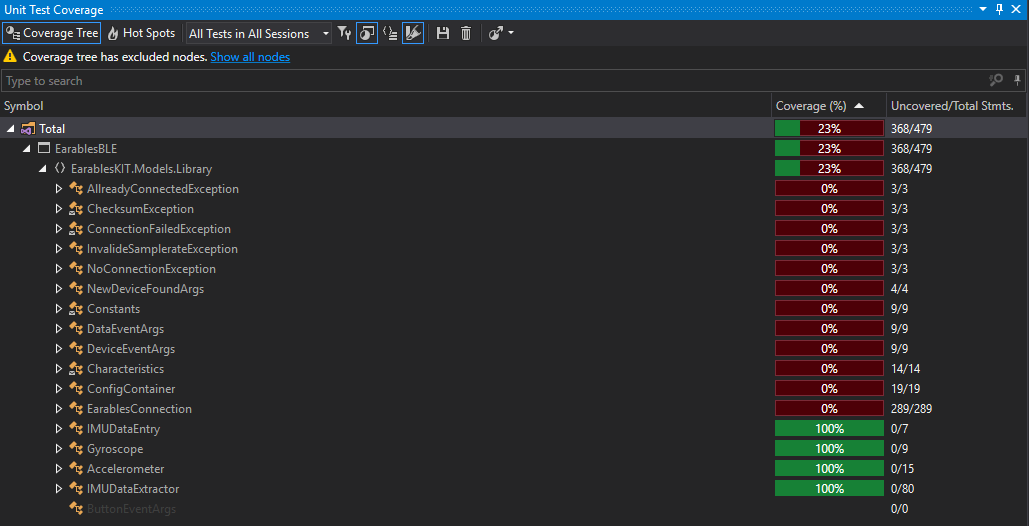
\includegraphics[width=1\textwidth]{./bilder/BibTestCoverage/Testcoverage.PNG}
\subsection{Model}
Bei unserm Model haben wir nahezu alles getestet. Die Algorithmen haben wir mit voraufgezeichneten Daten gefüttert und gezählt wie viele Aktivitäten der Algorithmus erkannt hat. So konnten wir die Algorithmen mit gemockten Daten auf Korrektheit testen. Vergleichbar ist dies mit dem SettingsService. \\Zudem haben wir bei allen Tests mit der internen Reflection gearbeitet. Somit konnten wir den Serviceprovider im Servicemanager mocken. Über diesen können dann die gemockten Services zurückgegeben werden, damit die zu testende Klasse ohne Abhängigkeiten getestet werden kann.\\

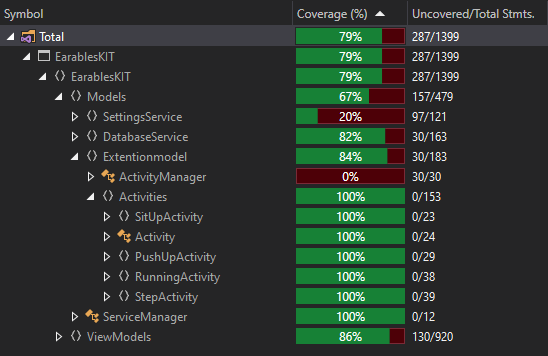
\includegraphics[width=1\textwidth]{./bilder/Coverage/CoverageModel.PNG}

\subsection{ViewModel}
Wir haben jedes ViewModel getestet. Dabei haben wir die 100\% Coverage angepeilt. Diese konnten wir nicht in jedem ViewModel erreichen, da es statische Methoden und Properties gibt, die nicht gemockt werden können. Bei diesen handelt es sich oft um spezifische Device Methoden. Auch im Viewmodel haben wir mit der internen Reflection gearbeitet, da jedes Viewmodel eine Relation zu mindestens einem anderen Service besitzt.\\
\newline
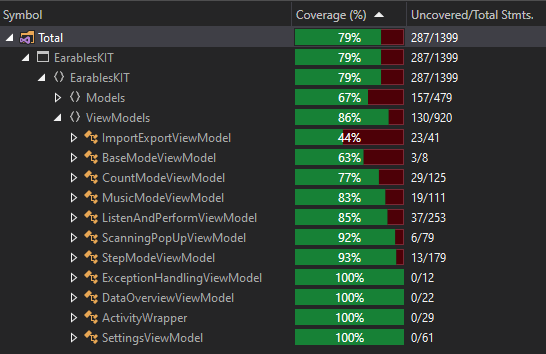
\includegraphics[width=1\textwidth]{./bilder/Coverage/CoverageViewModels.PNG}

\section{Test App für die Bibliothek}
\subsection{Motivation}
Die Bibliothek wird als NuGet-Package veröffentlicht. Daher wollten wir besonders hier einen hohen Wert auf die Korrektheit legen und umfassend testen.\\
Da wir für die Bluetoothverbindung in unserer Bibliothek das NuGet \glqq{}lBluetooth LE plugin for Xamarin\grqq{} benutzen, erschwert uns dies das Testen mit xUnit tests. Wir können hier nicht, wie beim Rest des Projektes, mit Reflection arbeiten, weil es sich bei der \glqq{}obersten Klasse\grqq{} um eine static Klasse handelt. Diese besitzt nur eine static Property, welche man nicht mocken kann, da kein Setter bereitstellt wird.\\
 Um unsere Bibliothek trotzdem zu testen, haben wir uns dafür entschieden eine eigene Test App für die Bibliothek zu bauen. So sind wir in der Lage, mit kleine Szenarien, die nur unsere Bibliothek betreffen, zielgerichtete Tests durchzuführen.
 \subsection{Funktionsweise}
Mit der Test App werden alle Funktionalitäten getestet, die die Bibliothek bereitstellt. Diese sind:
\begin{itemize}
	\item das Suchen von Geräten über Bluetooth
	\item das Verbinden mit Bluetooth Geräten (speziell mit Earables)
	\item das Trennen von Bluetooth Geräten
	\item das Setzen des LPF für das Gyroskop
	\item das Auslesen des LPF für das Gyroskop
	\item das Setzen des LPF für den Accelerometer
	\item das Auslesen des LPF für den Accelerometer
	\item das Starten des Samplings
	\item das Stoppen des Samplings
	\item das Setzen der Samplingrate
	\item das Auslesen der Samplingrate
	\item das Setzen der Range des Gyroskops
	\item das Auslesen des Scalefactors für das Gyroskop (hängt von der Range ab und wird für die Erzeugung der Rohdaten benötigt)
	\item das Setzen der Range des Accelerometers
	\item das Auslesen des Scalefactors für den Accelerometer (hängt von der Range ab und wird für die Erzeugung der Rohdaten benötigt)
	\item das Anzeigen der Battery Voltage und das Ermitteln des Verbindungdsstatuses
\end{itemize}

\subsection{Testszenarien}
Da da Test App für die Bibliothek nicht in der Definitionsphase geplant wurde, sondern nur zum Testen in der Testphase geschrieben wurde, mussten hier neue Testszenarien entwickelt werden. Diese sind im Folgenden mit Testergebnis aufgeführt. Die geteste Funktionalität umfasst die Anforderungen aus dem Pflichtenheft sehr ausführlich und detailreich.
\subsubsection{Verbinden mit den Earables}
\begin{tabular}{ | p{12cm} | c| }
	\hline
	\textbf{Beschreibung} & \textbf{Bestanden}\\
	\hline
	Der Nutzer startet die App. &\testok \\
	\hline
	Der Nutzer drückt den Button \glqq{}Get  connection status\grqq{}. & \testok \\
	\hline
	Es erscheint ein Pop-up welches als connection status \glqq{}getrennt\grqq{} anzeigt. & \testok \\
	\hline
	Der Nutzer klickt das Pop-up weg. & \testok \\
	\hline
	Der Nutzer drückt den Button \glqq{}Search\grqq{}. & \testok \\
	\hline
	Der Nutzer wählt seine Earables, als zu verbindendes Device, aus. & \testok \\
	\hline
	Es erscheint ein Pop-up, das dem Nutzer anzeigt, dass er nun, mit den Earables verbund ist. & \testok \\
	\hline
	Der Nutzer klickt das Pop-up weg. & \testok \\
	\hline
	Der Nutzer drückt den Button \glqq{}Get  connection status\grqq{}. & \testok \\
	\hline
	Es erscheint ein Pop-up welches als connection status \glqq{}verbunden\grqq{} anzeigt. & \testok \\
	\hline
	Der Nutzer klickt das Pop-up weg. & \testok \\
	\hline
	Der Nutzer drückt den Button \glqq{}Disconnect\grqq{}. & \testok \\
	\hline
	Es erscheint ein Pop-up welches als connection status \glqq{}getrennt\grqq{} anzeigt. & \testok \\
	\hline
	Der Nutzer klickt das Pop-up weg. & \testok \\
	\hline
	Der Nutzer drückt den Button \glqq{}Get  connection status\grqq{}. & \testok \\
	\hline
	Es erscheint ein Pop-up welches als connection status \glqq{}getrennt\grqq{} anzeigt. & \testok \\
	\hline
	Der Nutzer klickt das Pop-up weg. & \testok \\
	\hline
\end{tabular}



\begin{figure}
    \subfigure[App nach dem Starten]{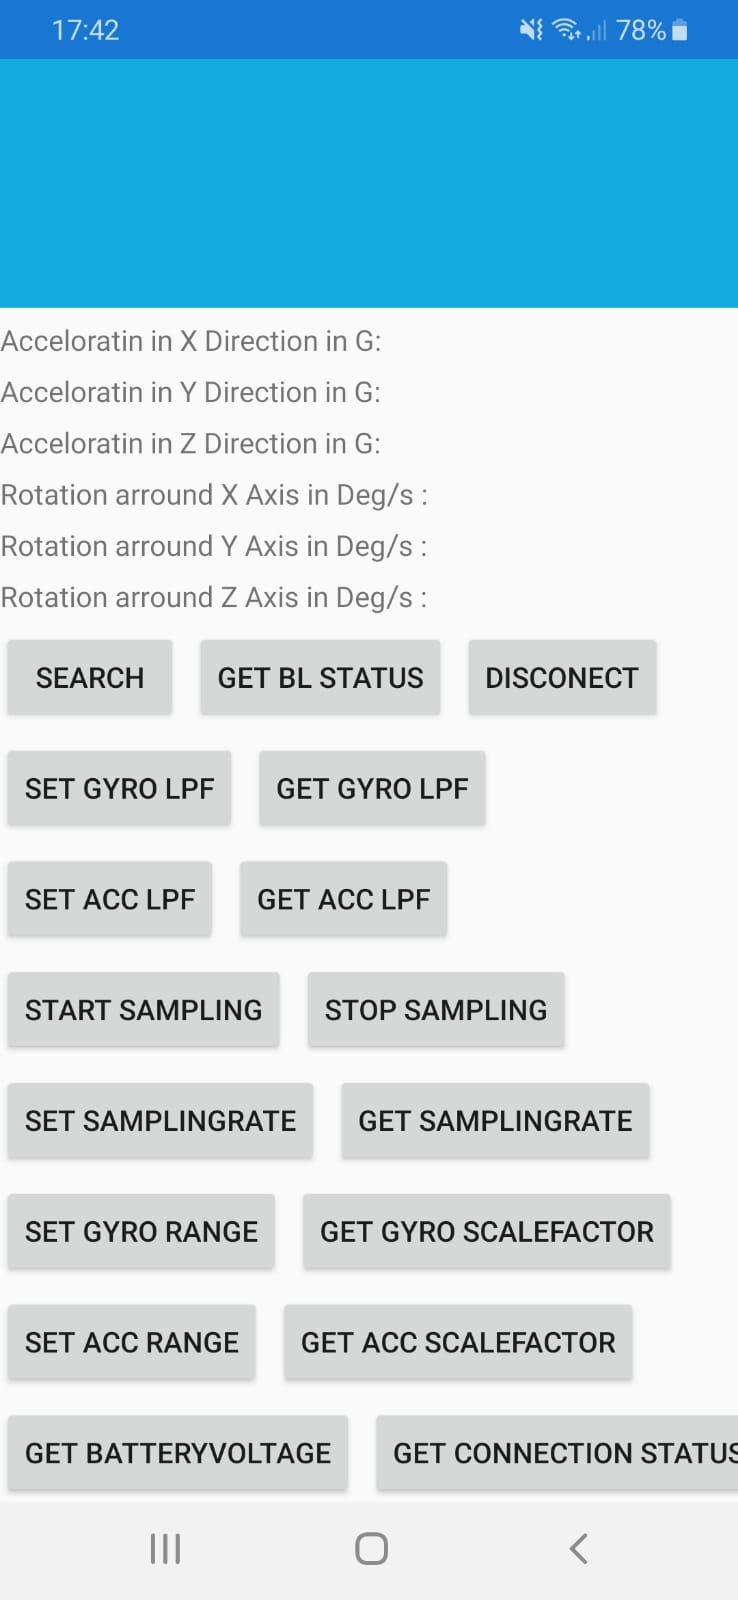
\includegraphics[width=0.4\textwidth]{./bilder/BibTestApp/Start.jpeg}}
   \hfill
    \subfigure[App nach dem Verbinden mit den Earables]{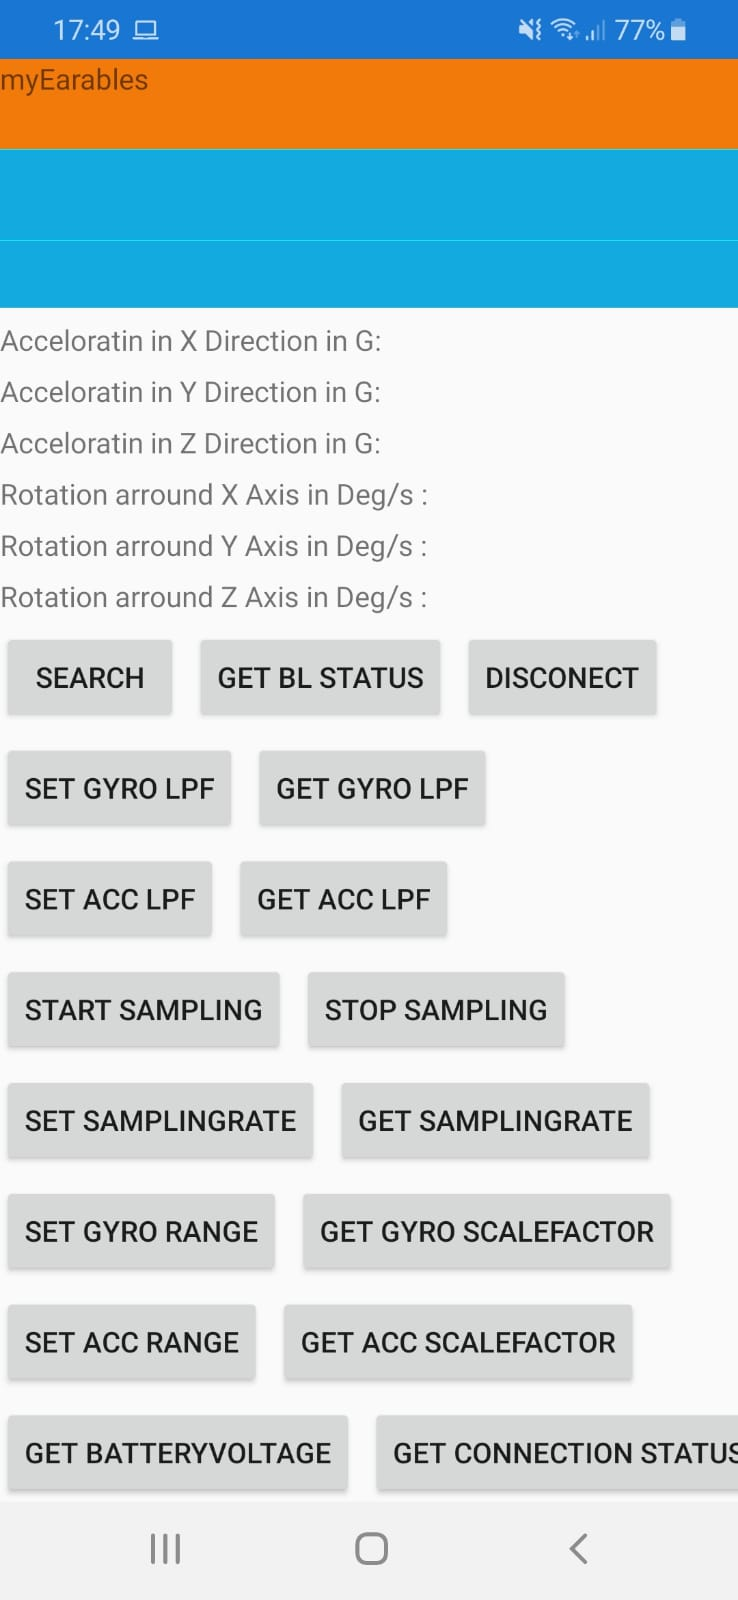
\includegraphics[width=0.4\textwidth]{./bilder/BibTestApp/Connect.jpeg}}
\end{figure}
\FloatBarrier

Hinweis: Für die nachfolgenden Szenarien wird angenommen, dass die App bereits gestartet ist und eine Verbindung zu den Earable besteht.

\subsubsection{Sampling starten}
\begin{tabular}{ | p{12cm} | c| }
	\hline
	\textbf{Beschreibung} & \textbf{Bestanden}\\
	\hline
	Der Nutzer drückt den Button \glqq{}Start Sampling\grqq{}. & \testok \\
	\hline
	Es werden die Rohdaten auf dem Bildschirm angezeigt. & \testok \\
	\hline
	Der Nutzer bewegt seinen Kopf und sieht wie sich die Rohdaten dementsprechend verändern. & \testok \\
	\hline
	Der Nutzer drückt den Button \glqq{}Stop Sampling\grqq{}. & \testok \\
	\hline
	Das Sampling wird gestoppt und die Rohdaten hören auf sich zu aktualisieren. & \testok \\
	\hline
\end{tabular}
\\ \\ \\ \\
\begin{figure}[h]
	\centering
    \subfigure[App zeichnet Daten auf]{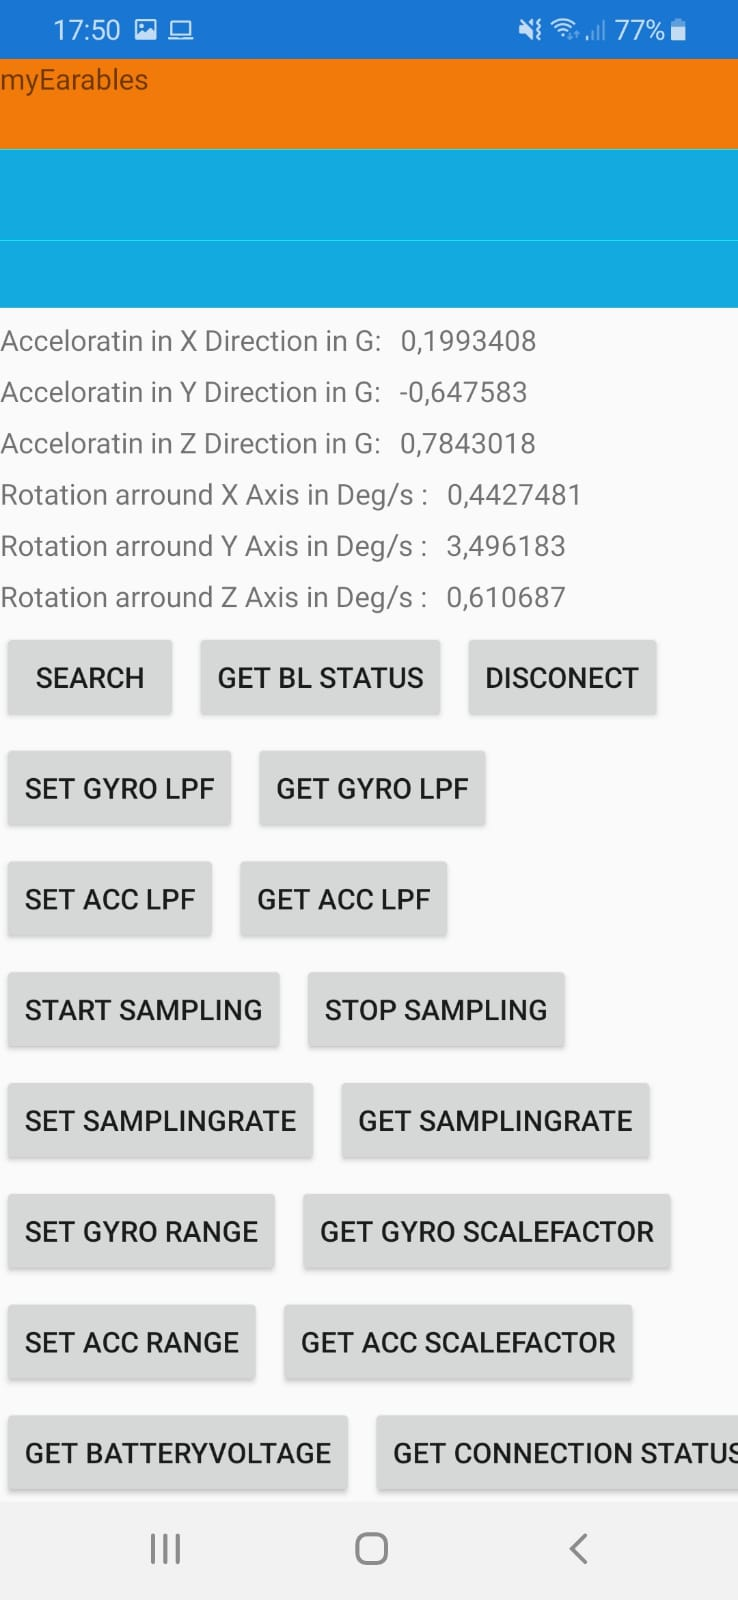
\includegraphics[width=0.4\textwidth]{./bilder/BibTestApp/StartSampling.jpeg}}
\end{figure}
\FloatBarrier

\subsubsection{Setzen des LPF für das Gyroscope}
\begin{tabular}{ | p{12cm} | c| }
	\hline
	\textbf{Beschreibung} & \textbf{Bestanden}\\
	\hline
	Der Nutzer drückt den Button \glqq Get Gyro LPF\grqq{}. & \testok \\
	\hline
	Es wird angezeigt dass der LPF für das Gyroscope 5Hz beträgt . & \testok \\
	\hline
	Der Nutzer drückt den Button \glqq Set Gyro LPF\grqq{}. & \testok \\
	\hline
	Der Nutzer wählt 41Hz als LPF aus. & \testok \\
	\hline
	Es wird angezeigt, dass der LPF auf 41Hz gesetzt wird . & \testok \\
	\hline
	Der Nutzer drückt den Button \glqq Get Gyro LPF\grqq{}. & \testok \\
	\hline
	Es wird angezeigt, dass der LPF für das Gyroscope 41Hz beträgt . & \testok \\
	\hline
\end{tabular}
\\ \\ \\ \\
\begin{figure}[h]
	\centering
    \subfigure[App fordert den Nutzer, nach drücken des Buttons \glqq{Set Gyro LPF}, auf einen LPF für das Gyroscope  auszuwählen]{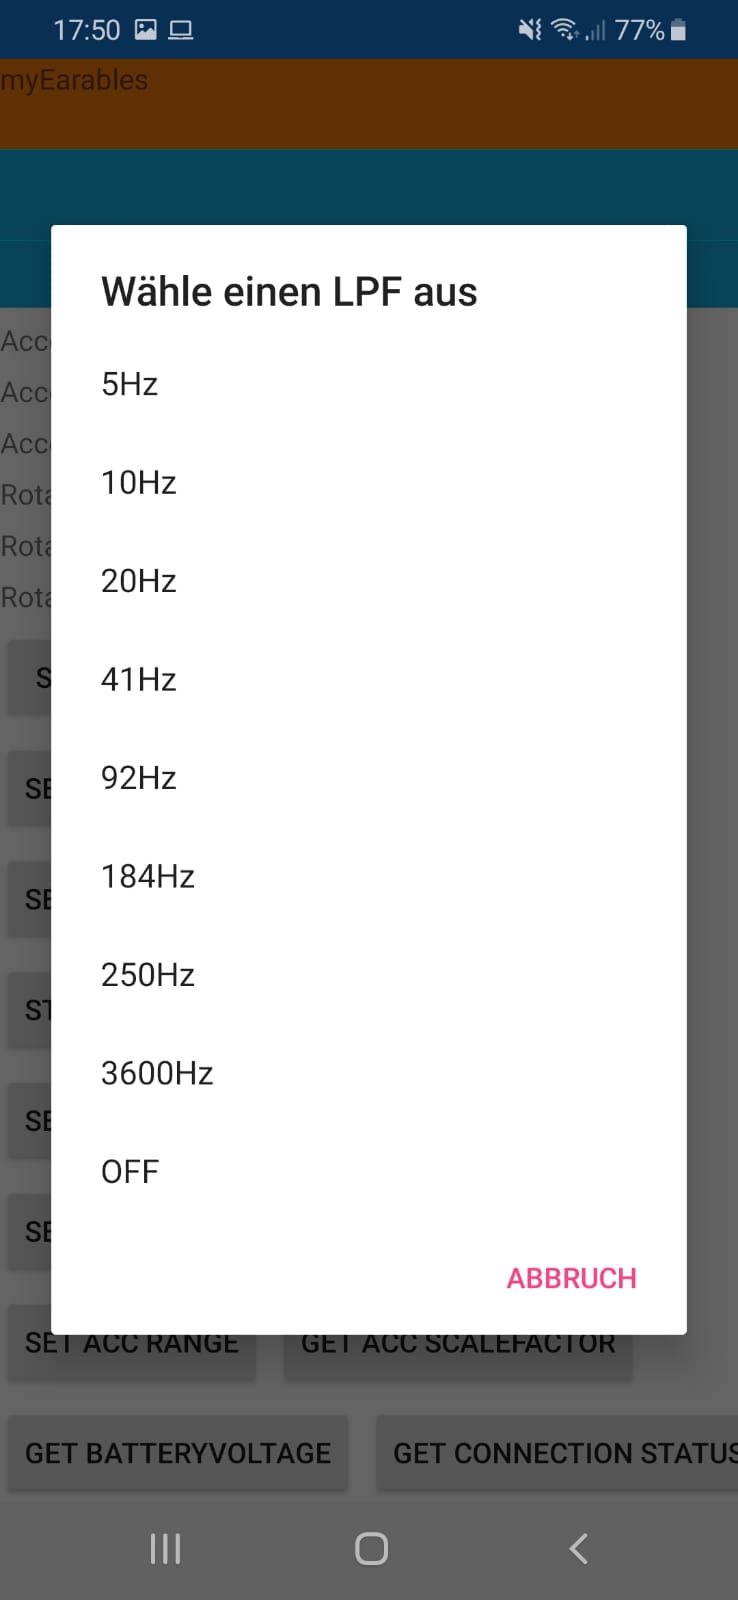
\includegraphics[width=0.4\textwidth]{./bilder/BibTestApp/GyroLPF.jpeg}}
\end{figure}
\FloatBarrier

\subsubsection{Setzen des LPF für den Accelerometer}
\begin{tabular}{ | p{12cm} | c| }
	\hline
	\textbf{Beschreibung} & \textbf{Bestanden}\\
	\hline
	Der Nutzer drückt den Button \glqq Get Acc LPF\grqq{}. & \testok \\
	\hline
	Es wird angezeigt dass der LPF für den Acc 5Hz beträgt . & \testok \\
	\hline
	Der Nutzer drückt den Button \glqq Set Acc LPF\grqq{}. & \testok \\
	\hline
	Der Nutzer wählt 184Hz als LPF aus. & \testok \\
	\hline
	Es wird angezeigt, dass der LPF auf 184Hz gesetzt wird . & \testok \\
	\hline
	Der Nutzer drückt den Button \glqq{}Get Acc LPF\grqq{}. & \testok \\
	\hline
	Es wird angezeigt, dass der LPF für den Accelerometer 41Hz beträgt . & \testok \\
	\hline
\end{tabular}
\\ \\ \\ \\
\begin{figure}[h]
	\centering
    \subfigure[App fordert den Nutzer, nach drücken des Buttons \glqq{Set Acc LPF}, auf einen LPF für den Accelerometer auszuwählen]{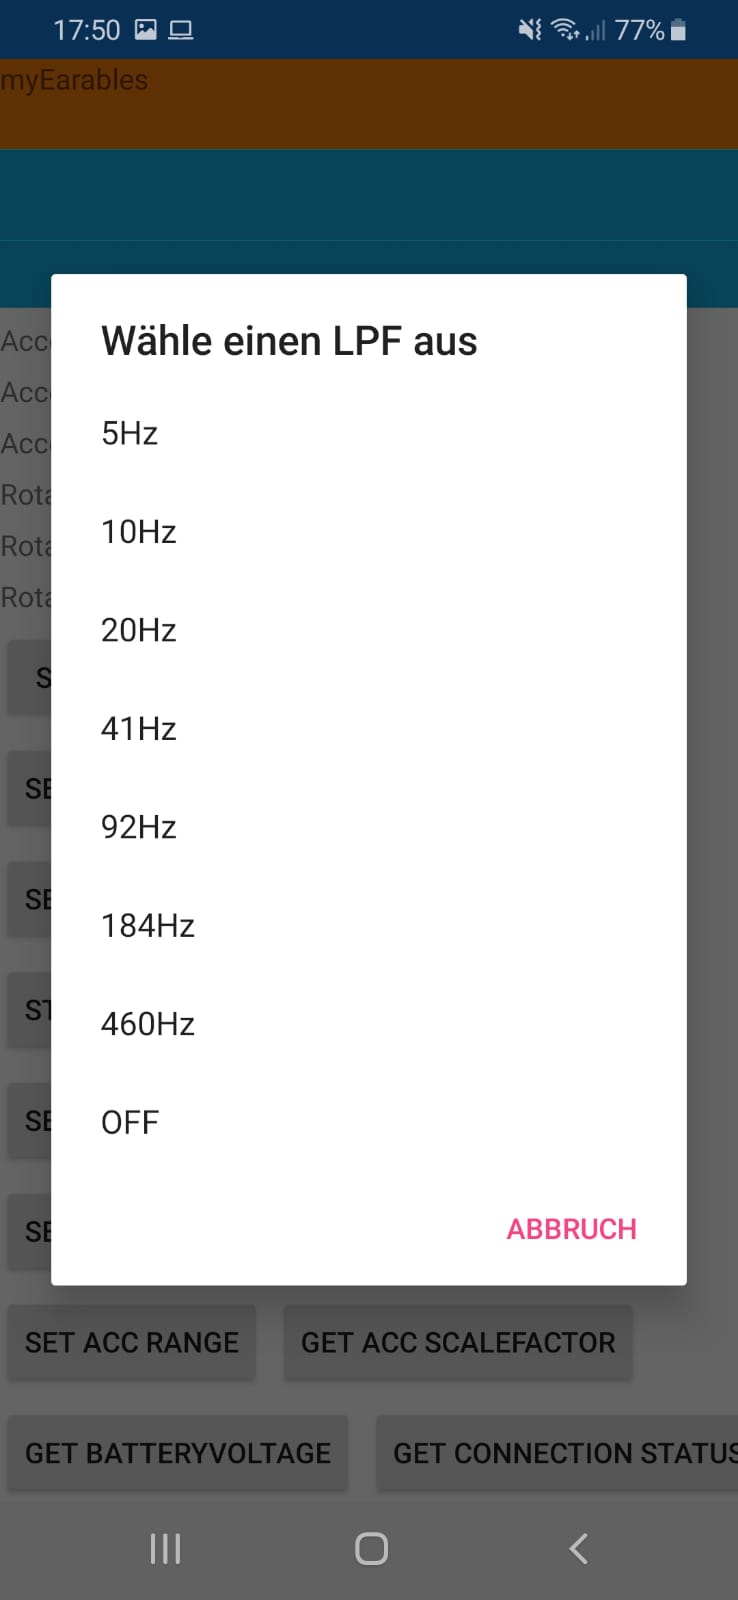
\includegraphics[width=0.4\textwidth]{./bilder/BibTestApp/AccLPF.jpeg}}
\end{figure}
\FloatBarrier

\subsubsection{Samplingrate verändern}
\begin{tabular}{ | p{12cm} | c| }
	\hline
	\textbf{Beschreibung} & \textbf{Bestanden}\\
	\hline
	Der Nutzer drückt den Button \glqq{}Start Sampling\grqq{}. & \testok \\
	\hline
	Es werden die Rohdaten auf dem Bildschirm angezeigt und der Nutzer sieht, dass sie sich 50 mal pro Sekunde aktualisieren. & \testok \\
	\hline
	Der Nutzer bewegt seinen Kopf und sieht wie sich die Rohdaten dementsprechend verändern. & \testok \\
	\hline
	Der Nutzer drückt den Button \glqq{}Stop Sampling\grqq{}. & \testok \\
	\hline
	Das Sampling wird gestoppt und die Rohdaten hören auf sich zu aktualisieren. & \testok \\
	\hline
	Der Nutzer drückt den Button \glqq{}Get Samplingrate\grqq{}. & \testok \\
	\hline
	Es wird angezeigt dass die Samplingrate 50Hz beträgt. & \testok \\
	\hline
	Der Nutzer drückt den Button \glqq{}SetSamplingrate\grqq{}. & \testok \\
	\hline
	Der Nutzer gibt 1 als Samplingrate ein. & \testok \\
	\hline
	Es wird angezeigt, dass die Samplingrate auf 1 gesetzt wird. & \testok \\
	\hline
	Der Nutzer drückt den Button \glqq{}Start Sampling\grqq{}. & \testok \\
	\hline
	Es werden die Rohdaten auf dem Bildschirm angezeigt und der Nutzer sieht, dass sie sich nur ein mal pro Sekunde aktualisieren. & \testok \\
	\hline
	Der Nutzer bewegt seinen Kopf und sieht wie sich die Rohdaten dementsprechend verändern. & \testok \\
	\hline
	Der Nutzer drückt den Button \glqq{}Stop Sampling\grqq{}. & \testok \\
	\hline
	Das Sampling wird gestoppt und die Rohdaten hören auf sich zu aktualisieren. & \testok \\
	\hline
\end{tabular}
\\ \\ \\ \\
\begin{figure}[h]
	\centering
    \subfigure[App fordert den Nutzer, nach drücken des Buttons \glqq{Set Samplingrate}, auf eine gültige Samplingrate einzugeben]{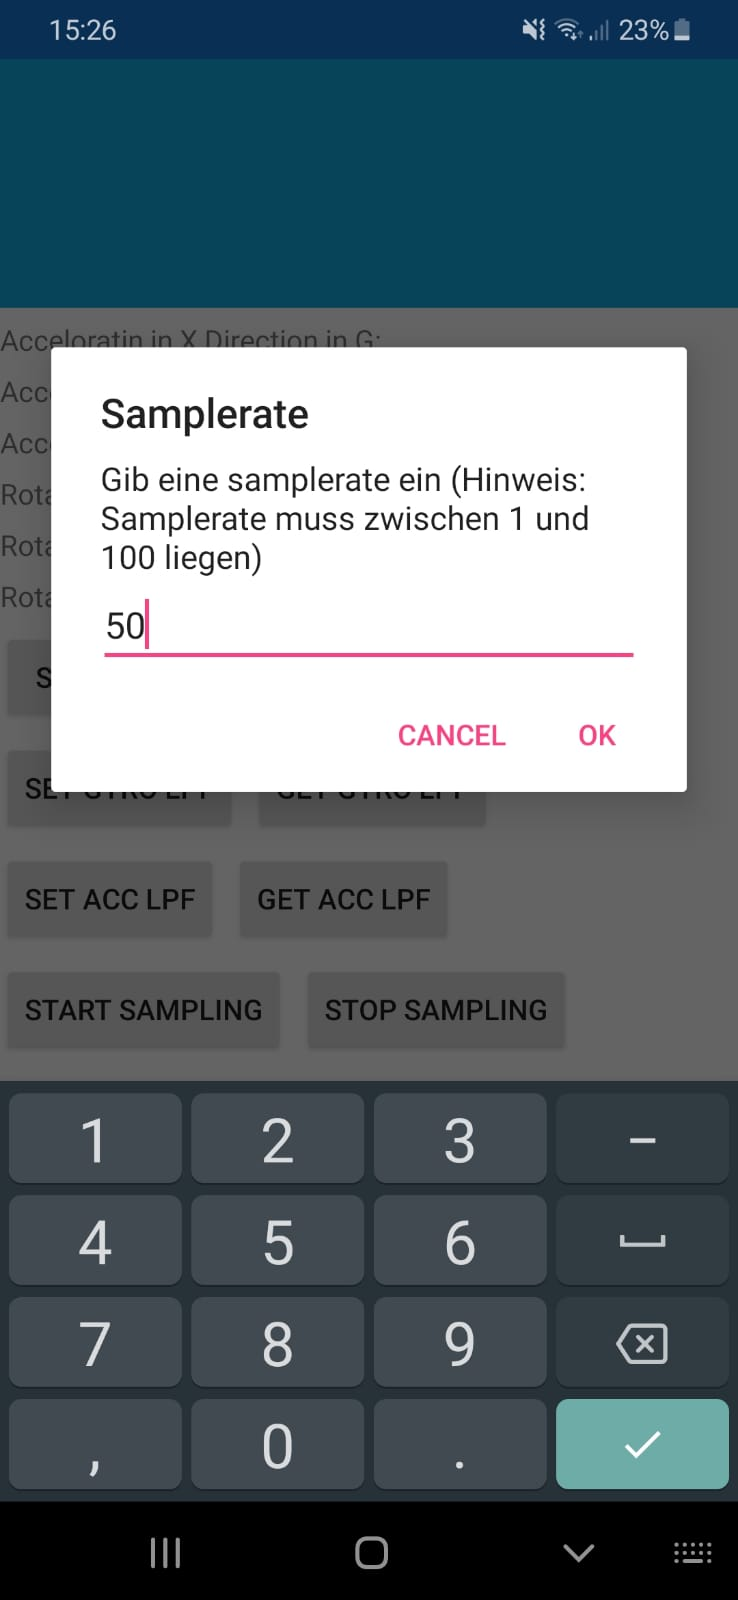
\includegraphics[width=0.4\textwidth]{./bilder/BibTestApp/SetSamplerate.jpeg}}
\end{figure}
\FloatBarrier

\subsubsection{Gyro Range verändern}
\begin{tabular}{ | p{12cm} | c| }
	\hline
	\textbf{Beschreibung} & \textbf{Bestanden}\\
	\hline
	Der Nutzer drückt den Button \glqq{}Get Gyro Scalefactor\grqq{}. & \testok \\
	\hline
	Es wird angezeigt, dass der Gyro Scale Factor 65,5 beträgt. & \testok \\
	\hline
	Der Nutzer drückt den Button \glqq{}Start Sampling\grqq{}. & \testok \\
	\hline
	Es werden die Rohdaten auf dem Bildschirm angezeigt und der Nutzer erkennt, dass die Range der Rotationen um die Achsen auf +- 500 deg/s beschrängt ist, wenn er seinen Kopf dreht. & \testok \\
	\hline
	Der Nutzer drückt den Button \glqq{}Stop Sampling\grqq{}. & \testok \\
	\hline
	Das Sampling wird gestoppt und die Rohdaten hören auf sich zu aktualisieren. & \testok \\
	\hline
	Der Nutzer drückt den Button \glqq{}Set Gyro Range\grqq{}. & \testok \\
	\hline
	Er wählt 250deg/s aus. & \testok \\
	\hline
	Es wird angezeigt, dass die Gyro Range jetzt 250deg/s beträgt. & \testok \\
	\hline
	Der Nutzer drückt den Button \glqq{}Get Gyro Scalefactor\grqq{}. & \testok \\
	\hline
	Es wird angezeigt, dass der Gyro Scale Factor 131 beträgt. & \testok \\
	\hline
	Der Nutzer drückt den Button \glqq{}Start Sampling\grqq{}. & \testok \\
	\hline
	Es werden die Rohdaten auf dem Bildschirm angezeigt und der Nutzer erkennt, dass die Range der Rotationen um die Achsen auf +- 250 deg/s beschrängt ist, wenn er seinen Kopf dreht. & \testok \\
	\hline
	Der Nutzer drückt den Button \glqq{}Stop Sampling\grqq{}. & \testok \\
	\hline
\end{tabular}
\\ \\
Hinweis: Der Scale Factor hängt von der gewählten Range ab.
\\ \\ \\ \\
\begin{figure}[h]
	\centering
    \subfigure[App fordert den Nutzer, nach drücken des Buttons \glqq{Set Gyro Range}, auf einen Range für das Gyroscope auszuwählen]{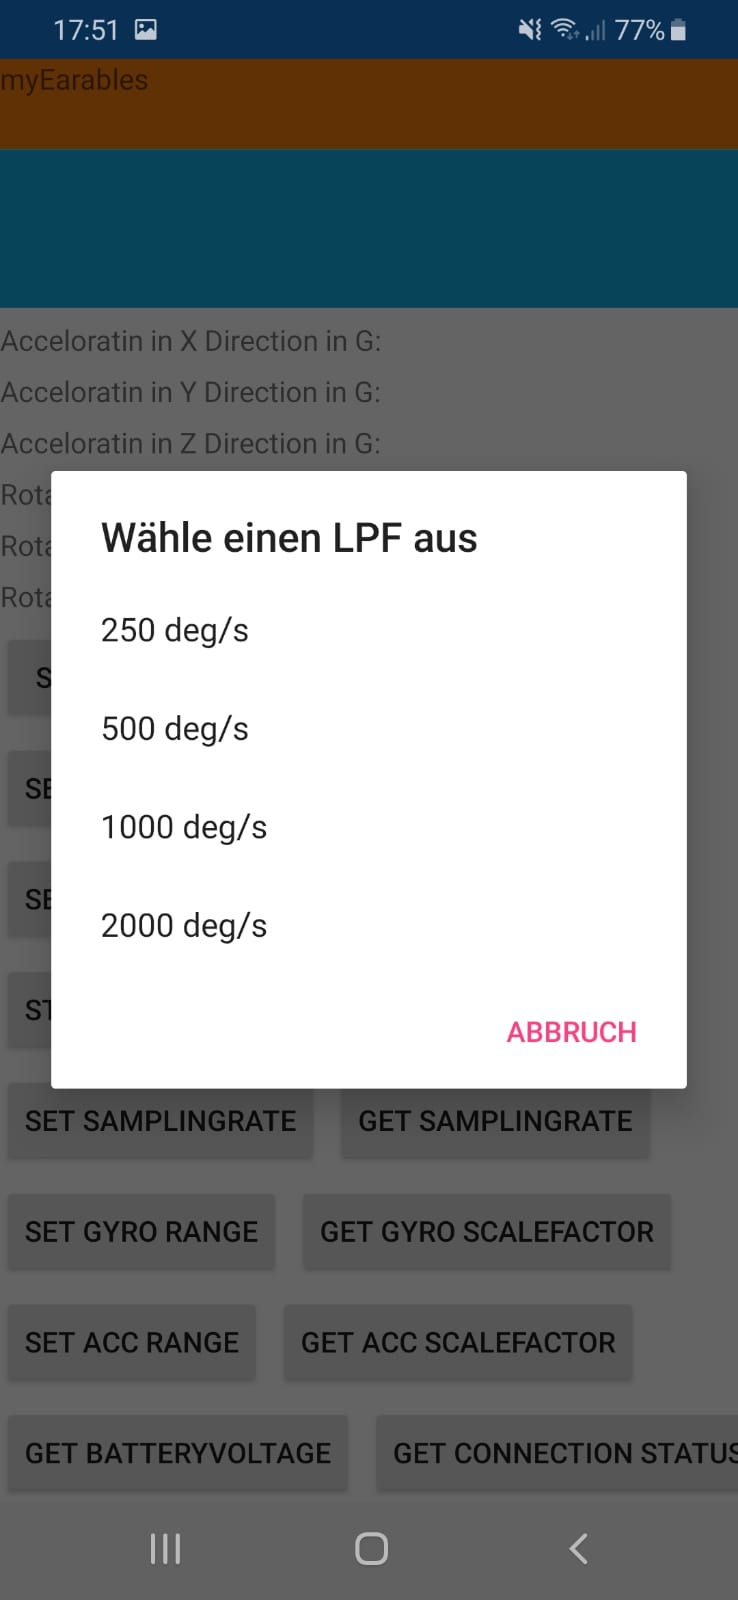
\includegraphics[width=0.4\textwidth]{./bilder/BibTestApp/GyroRange.jpeg}}
\end{figure}
\FloatBarrier

\subsubsection{Acc Range verändern}
\begin{tabular}{ | p{12cm} | c| }
	\hline
	\textbf{Beschreibung} & \textbf{Bestanden}\\
	\hline
	Der Nutzer drückt den Button \glqq{}Get Acc Scalefactor\grqq{}. & \testok \\
	\hline
	Es wird angezeigt, dass der Gyro Scale Factor 8192 beträgt. & \testok \\
	\hline
	Der Nutzer drückt den Button \glqq{}Start Sampling\grqq{}. & \testok \\
	\hline
	Es werden die Rohdaten auf dem Bildschirm angezeigt und der Nutzer erkennt, dass die Range der Beschleunigungen auf den Achsen  auf +-4 g beschränkt ist, wenn er sich bewegt. & \testok \\
	\hline
	Der Nutzer drückt den Button \glqq{}Stop Sampling\grqq{}. & \testok \\
	\hline
	Das Sampling wird gestoppt und die Rohdaten hören auf sich zu aktualisieren. & \testok \\
	\hline
	Der Nutzer drückt den Button \glqq{}Set Acc Range\grqq{}. & \testok \\
	\hline
	Er wählt 2g aus. & \testok \\
	\hline
	Es wird angezeigt, dass die Gyro Range jetzt 2g beträgt. & \testok \\
	\hline
	Der Nutzer drückt den Button \glqq{}Get Acc Scalefactor\grqq{}. & \testok \\
	\hline
	Es wird angezeigt, dass der Acc Scale Factor 16384 beträgt. & \testok \\
	\hline
	Der Nutzer drückt den Button \glqq{}Start Sampling\grqq{}. & \testok \\
	\hline
	Es werden die Rohdaten auf dem Bildschirm angezeigt und der Nutzer erkennt, dass die Range der Beschleunigungen auf den Achsen  auf +-2g beschränkt ist, wenn er sich bewegt. & \testok \\
	\hline
	Der Nutzer drückt den Button \glqq{}Stop Sampling\grqq{}. & \testok \\
	\hline
\end{tabular}
\\ \\
Hinweis: Der Scale Factor hängt von der gewählten Range ab.
\\ \\ \\ \\
\begin{figure}[h]
	\centering
    \subfigure[App fordert den Nutzer, nach drücken des Buttons \glqq{Set Acc Range}, auf einen Range für den Accelerometer auszuwählen]{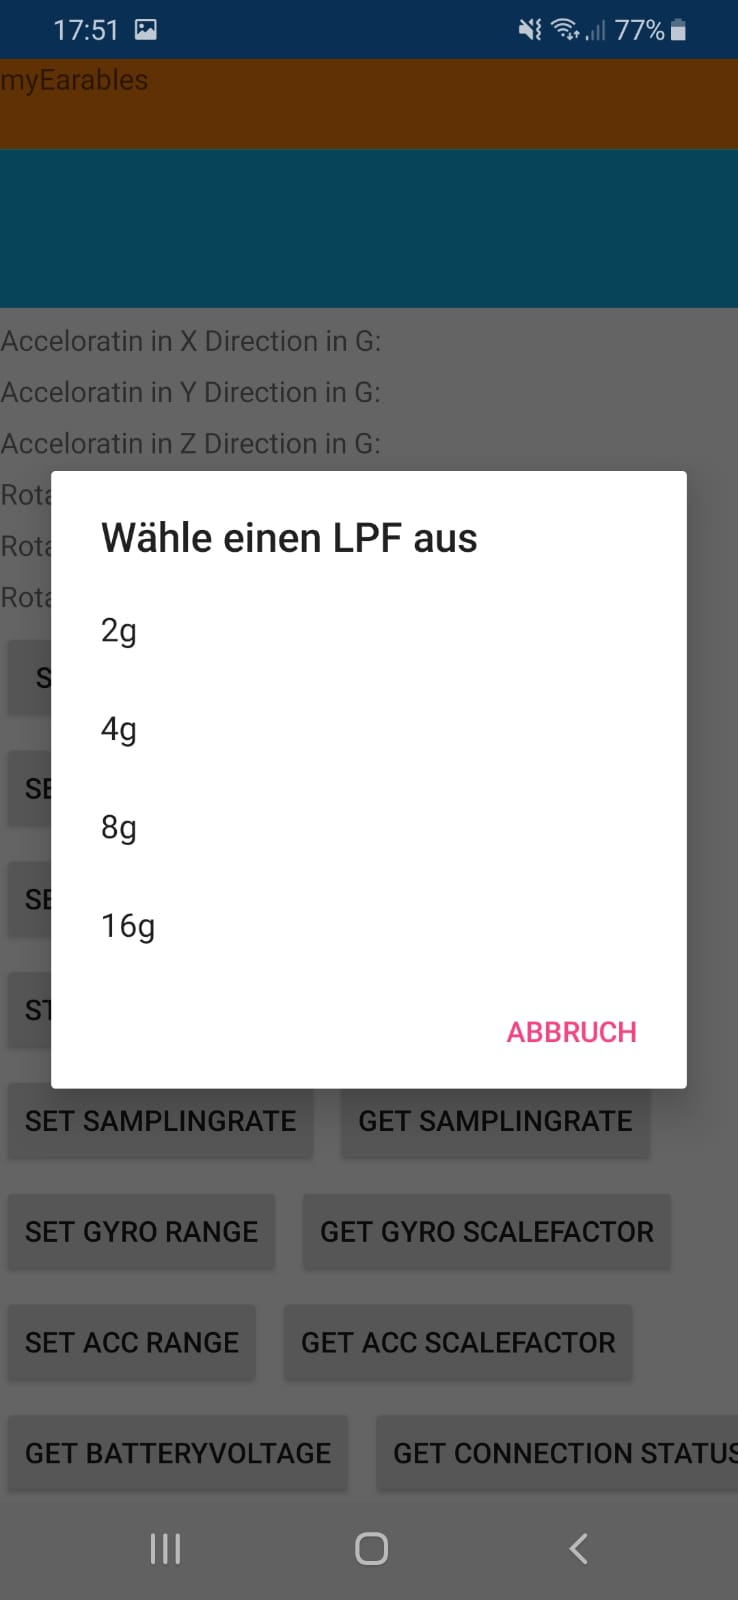
\includegraphics[width=0.4\textwidth]{./bilder/BibTestApp/AccRange.jpeg}}
\end{figure}
\FloatBarrier

\subsubsection{BatteryVoltage auslesen}
\begin{tabular}{ | p{12cm} | c| }
	\hline
	\textbf{Beschreibung} & \textbf{Bestanden}\\
	\hline
	Der Nutzer drückt den Button \glqq{}Get Batteryvoltage\grqq{}. & \testok \\
	\hline
	Es wird die aktuelle Batteryvoltage angezeigt. & \testok \\
	\hline
\end{tabular}
\\ \\ \\ \\
\begin{figure}[h]
	\centering
    \subfigure[App zeigt dem Nutzer, nach drücken des Buttons \glqq{Set Battervoltage}, den aktuellen Wert der Batterievotage an]{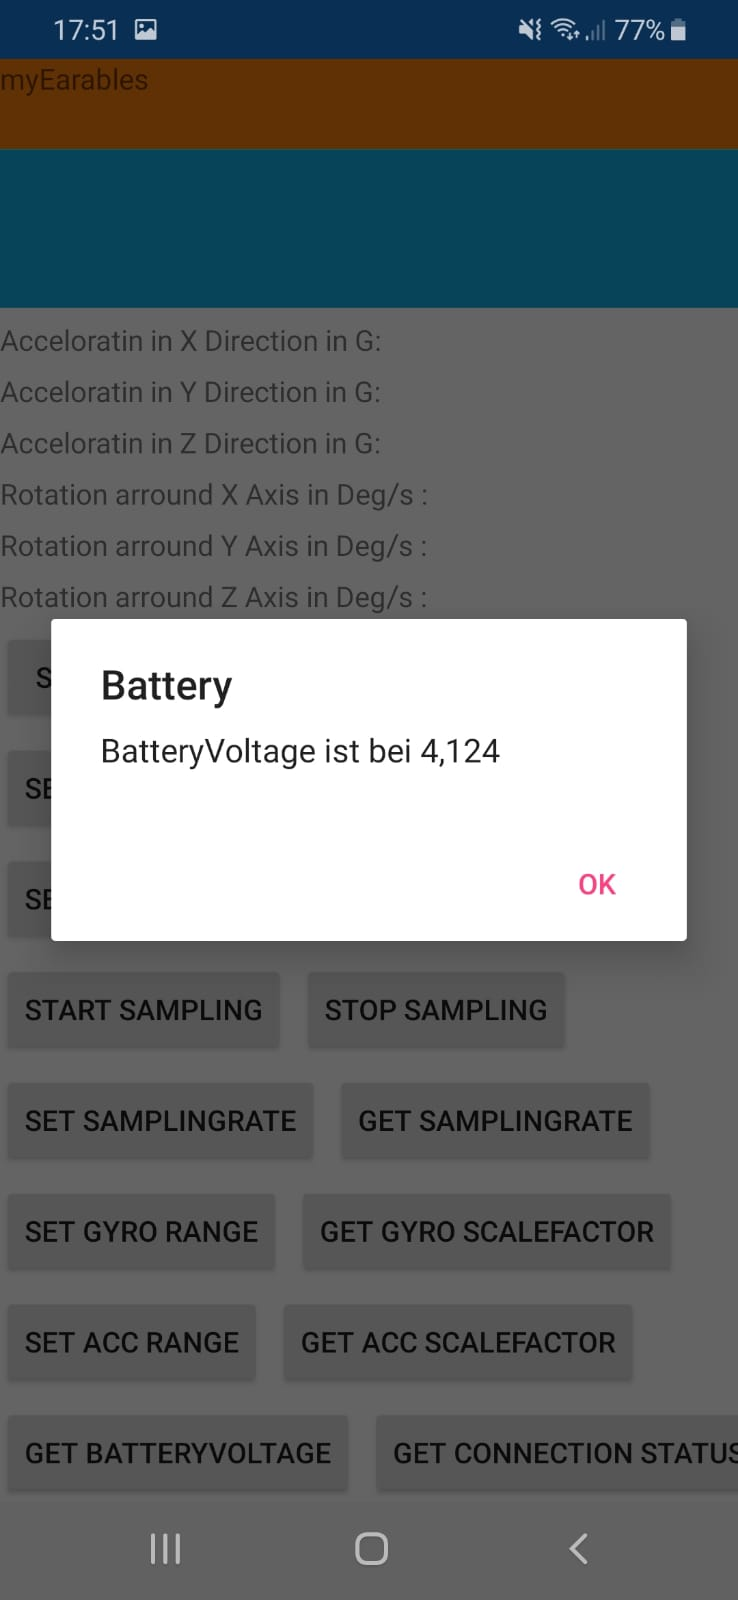
\includegraphics[width=0.4\textwidth]{./bilder/BibTestApp/BatteryVoltage.jpeg}}
\end{figure}
\FloatBarrier

\subsubsection{Push Button drücken}
\begin{tabular}{ | p{12cm} | c| }
	\hline
	\textbf{Beschreibung} & \textbf{Bestanden}\\
	\hline
	Der Nutzer drückt den Knopf an den Earables. & \testok \\
	\hline
	Auf der Console, im Debug Modus, wird eine Zeile ausgegeben, die dem Nutzer mitteilt, dass der Knopf an den Earables gedrückt wurde. & \testok \\
	\hline
\end{tabular}

\subsubsection{Bluetooth Status auslesen}
\begin{tabular}{ | p{12cm} | c| }
	\hline
	\textbf{Beschreibung} & \textbf{Bestanden}\\
	\hline
	Der Nutzer drückt den Button \glqq{}Get Bl status\grqq{}. & \testok \\
	\hline
	Es wird angezeigt, dass Bluetooth am Handy eingeschaltet ist. & \testok \\
	\hline
	Der Nutzer schaltet Bluetooth an seinem Smartphone aus. & \testok \\
	\hline
	Der Nutzer drückt den Button \glqq{}Get Bl status\grqq{}. & \testok \\
	\hline
	Es wird angezeigt, dass Bluetooth am Handy ausgeschaltet ist. & \testok \\
	\hline
\end{tabular}

\section{Nutzertests}
\paragraph{Einleitung}
Diese Tests wurden mit Testpersonen ausgeführt, die nicht an der Entwicklung der App beteiligt waren. Wir haben dabei fünf Testpersonen ($P_1 \text{ bis } P_5$) die gleichen Abläufe in der App durchlaufen lassen.
\paragraph{Vorbereitung}
Die Verbindung zu den Earables wurde bereits vor dem Testdurchlauf hergestellt.
Die App wurde gestartet.\\
An die Tespersonen wurden folgende Hinweise gegeben:
\begin{itemize}
	\item Der Modus soll erst in Startposition gestartet werden.
	\item Situps sollen so ausführt werden, wie es vorgemacht wird (Bewegung vom Boden aus bis in die aufrechte Sitzposition)
	\item Vor jedem Test wird der Testperson mitgeteilt, welcher Modus und wie viele Wiederholungen gemacht werden sollen.
	\item Beim Zählen der Schritte sollte \textit{zügig gegangen} werden, nicht gerannt oder geschlendert (damit die Tests einheitlich sind).
\end{itemize}

\subsection{Zählmodus}
\subsubsection{10 Liegestützen}
%hier Kommentare zu euren Testpersonen ergänzen
Bei $P_1$ wurden alle Liegestütze beim ersten Mal erkannt.\\
Bei $P_2$ wurden die ersten 3 Liegestütze zu schnell durchgeführt weswegen sie nur als eine gezählt wurden.\\
Bei $P_4$ wurden alle Liegestütze beim ersten Mal erkannt.\\
Bei $P_5$ wurde die zweite Liegestütze nicht erkannt, die siebte dafür doppelt.\\
\subsubsection{10 SitUps}
%hier Kommentare zu euren Testpersonen ergänzen
Bei $P_1$ wurden die letzten beiden Sit-ups wegen unzureichender Bewegung in die aufrechte Sitzposition nicht erkannt.\\
Bei $P_2$ wurden die Sit-Ups sehr schlecht erkannt, obwohl die Ausführung korrekt war.\\
Bei $P_4$ gab es Probleme mit der korrekten Ausführung, weshalb mehr gemacht wurden mussten, sodass alle erkannt werden.\\
Bei $P_5$ musste die Übung wiederholt werden, da bei erstem Durchlauf die Verbindung zu den Kopfhöhrern abgebrochen ist.
\subsection{Laufmodus}
%hier Kommentare zu euren Testpersonen ergänzen
%bei P5 keine Kommentare
\subsubsection{30 Schritte am Stück}
%hier Kommentare zu euren Testpersonen ergänzen
Bei $P_1$ wurden die ersten 7 Schritte nicht erkannt, danach jedoch alle Weiteren.\\
Nachdem der Laufmodus beendet wurde und das Pop Up erschienen ist, ist die App, bei $P_2$  abgestürzt.\\
Bei $P_4$ wurde korrekt gemessen.\\
$P_5$ ist direkt nach Starten der Aktivität losgelaufen, trotzdem war das Ergebnis korrekt.
\subsubsection{20 Schritte, dann stoppen, dann wieder 20 Schritte}
Bei  $P_1$ und $P_4$ wurde korrekt gemessen. Das Stehenbleiben wurde beachtet und erkannt.\\
$P_5$ ist schon während dem Starten losgelaufen, hier wurden drei Schritte unterschlagen; das Stehenbleiben wurde korrekt erkannt, beim wieder Loslaufen wurde erneut ein Schritt unterschlagen.\\
\subsection{Listen And Perform}
\subsubsection{8 SitUps, 10 Sekunden Pause, 8 Liegestützen}
%hier Kommentare zu euren Testpersonen ergänzen
Bei $P_1$ verlief die Trainingsplanerstellung reibungslos, nur die Ausführung der fünften Liegestütze musste wiederholt werden.\\
Die Erstellung des Trainingsplans hat bei $P_2$ ohne Probleme funktioniert. Die Erkennung der Sit-Ups lief überdurchschnittlich schlecht ab. Es wurden, von 18 Sit-Ups, zwei erkannt. Der Test konnte nur dadurch fortgeführt werden, dass $P_2$ die Earables aus den Ohren genommen hat und die Sit-Up Bewegung simulierte, da $P_2$ keine Koordination mehr hatte. Die simulierten Sit-Ups wurden besser erkannt als die richtigen. Bei den Liegestützen hat $P_2$ die ersten 3 Liegestütze zu schnell durchgeführt weswegen sie nur als eine gezählt wurden.\\
$P_4$ hat seinen Trainingsplan selbstständig eingestellt und hat die Übungen durchgeführt. Die SitUps wurden nicht richtig erkannt; es waren 4 zu wenig. Diese wurden dann simuliert, um die weiteren Funktionen zu testen.\\
Bei $P_5$ hat das Einstellen des Trainingsplans selbstständig funktioniert, bei der Durchführung wurden drei SitUps unterschlagen. $P_5$ reagierte etwas verwirrt, dass der Trainingsplan diesen Schritt noch nicht vollständig abgearbeitet hatte.
\subsection{Statistik der Nutzertests}
\begin{tabular}{ | l | c | c | c | c | c | c |}
	\hline
	\textbf{Übung} & \textbf{Anzahl} & $P_1$ & $P_2$ & $P_3$ & $P_4$ & $P_5$\\
	\hline
	Liegestützen & 10 & 10 & 8 & 7 & 10 & 10 \\
	\hline
	SitUps & 10 & 8 & 4 & 3 & 7 & 9 \\
	\hline
	Schritte & 30 & 23 &25 & 34 & 30 & 30 \\
	\hline
	Schritte (mit stoppen) & 40 & 40 & 36 & 36 & 40 & 36 \\
	\hline
\end{tabular}\\
\paragraph{Anmerkungen}
%% @David vielleicht könnte man die Ergebnisse noch irgendwie kürzer zusammenfassen bzw. ein Toleranzniveau festlegen und alle ergebnisfelder dementsprechend grün / gelb / rot markieren
Da ListenAndPerform immer läuft, bis alle Bewegungen korrekt erkannt wurden, kann hier keine Statistik geliefert werden.


\section{Beschreibung Fehler}
%%david
\begin{itemize}
	\item[] \textsf{Szenario \glqq Zählmodus\grqq:} Die App zeigte nicht immer den korrekten Wert an.
										Das lag allerdings an dem Algorithmus, der bis zu 10\% Abweichung ermöglichte.
	\item[] \textsf{Szenario \glqq Einstellungen\grqq:} Die gespeicherten Vorgangsdaten können nicht in den Einstellungen gelöscht werden, sondern in der extra dafür vorgesehenen Seite \glqq Dateimanagemen\grqq.
	\item[] \textsf{Szenario \glqq Einstellungen\grqq:} Die Samplerate wird nicht gespeichert. Sie wird bei jedem Neustart der Kopfhörer zurück gesetzt.
	\item[] \textsf{Szenario \glqq Erstnutzung\grqq:} Bei der Erstnutzung wird der Nutzer nicht aufgefordert seinen Namen und seine Schrittlänge einzugeben.
	Diese Funktion wurde von uns entfernt, da sie nicht mehr benötigt wurde.
	\item[] \textsf{Szenario \glqq Vorgangsdaten importieren/exportieren\grqq:} Beim Löschen der Daten ist die App aus unbekannten Gründen abgestürzt.
\end{itemize}


\section{Anhang}
\subsection{Unit Test Reports}
\subsubsection{Bibliothek}
\subsubsection{App}

\subsection{Links}
\subsubsection{Bibliothek}
NuGet Package: \url{https://www.nuget.org/packages/EarablesBLE}\\
GitHub Repository: \url{https://github.com/vlle1/lib-earablesKIT}
\subsubsection{App und BibTestApp}
GitHub Repository: \url{https://github.com/vlle1/earablesKIT}
%%%%%%%%%%%%%%%%%%%%%%%%%%%%%%%%%%%%%%% END CONTENT %%%%%%%%%%%%%%%%%%%%%%%%%%%%%%%%%%%%%%%%%%%


\printglossaries
\stepcounter{section}


\end{document}